\documentclass[twoside,11pt]{article}

% Any additional packages needed should be included after jmlr2e.
% Note that jmlr2e.sty includes epsfig, amssymb, natbib and graphicx,
% and defines many common macros, such as 'proof' and 'example'.
%
% It also sets the bibliographystyle to plainnat; for more information on
% natbib citation styles, see the natbib documentation, a copy of which
% is archived at http://www.jmlr.org/format/natbib.pdf

\usepackage{jmlr2e}
\usepackage{graphicx}% Definitions of handy macros can go here
\usepackage{hyperref}


% Heading arguments are {volume}{year}{pages}{submitted}{published}{author-full-names}

\jmlrheading{1}{2009}{1-4}{2/09}{10/09}{Brian Tanner and Adam White}

% Short headings should be running head and authors last names

\ShortHeadings{RL-Glue}{Tanner and White}
\firstpageno{1}

\begin{document}

\title{RL-Glue : Language-Independent Software for Reinforcement-Learning Experiments}


\author{\name Brian Tanner \AND Adam White  \email \{btanner,awhite\}@cs.ualberta.ca \\
       \addr Department of Computing Science\\
       University of Alberta\\
       Edmonton, AB 98195-4322, Canada}

\editor{ Soeren Sonnenburg}

\maketitle

\begin{abstract}%
RL-Glue (Reinforcement-Learning Glue) provides a standard programming interface for learning experiments, even if the agent and environment are written in different languages. 
The standardization provided by RL-Glue facilitates code sharing and collaboration, reducing the need to re-engineer tasks and experimental apparatus from the literature in order to compare to and verify the results of others.
RL-Glue is well suited for empirical research, course work and industrial-scale projects. Our software features a minimalist interface and supports C, C++, Java, Python, Matlab and Lisp and runs on many computing platforms including Linux, Mac OS X and Microsoft Windows. RL-Glue can be easily extended to support additional programming languages and other evaluation software using a TCP/IP interface. RL-Glue has been used to teach classes, to evaluate participants during international reinforcement-learning competitions and is currently used by several other open-source software and hardware projects.
\end{abstract}

\section{Introduction and Motivation}
Reinforcement learning is an embodied, trial-and-error problem formulation for artificial intelligence~\citep{rlbook, rlsurvey,ndp}.  At a series of time steps, the {\it agent} emits actions in response to observations and rewards that have been generated by the {\it environment}.  The objective is to select actions that maximize some notion of the future rewards.  Reinforcement-learning methods have been successfully applied to many problems including Backgammon, helicopter flight, elevator control, automobile traffic flow control, and computer Go~\citep{rlbook}. Outside of machine learning, reinforcement-learning models and formalisms have influenced operations research, psychology, neuroscience, and others.


\textbf{We have a small issue here because the book doesn't talk about helicopter.  So we should cite Ng. Maybe we should cite something fresher, like Doug Aberdeen's traffic-light control stuff in Australia and Go?}


Reinforcement-learning environmentscannot be stored as a fixed data-set, as is common in conventional supervised learning.  The environment generates observations and reward in response to the action selected by the agent, making it more natural to think of the environment and agent as interactive ``programs'' instead of fixed data-sets.  Different members of the reinforcement-learning community create these agent and environment programs using various incompatible software frameworks, making collaboration difficult and thus slowing progress in our community. It  can be time consuming, difficult, and sometimes even impossible to exactly reproduce the work of others.  There is simply not enough space in the course of a conference publication to share a detailed specification of the environment, the agent, and the overall experimental apparatus.
In the most extreme cases, the source code for some reinforcement-learning environments has become publicly available in different variations that are still each referred to, in the literature, as ``the standard", ``well-known" or ``classical"  versions \citep{whiteThesis}.

We believe that a standard programming interface for reinforcement-learning experiments will remove some barriers to collaboration and accelerate the pace of research in reinforcement learning.  To encourage widespread adoption, this interface should be easy to adhere to, and it should not force users to abandon their favorite tools or languages.  With these goals in mind, we have developed the RL-Glue Software Project: a language independent interface for reinforcement-learning experiments.

%In reinforcement learning, an {\it agent} learns from the consequences of its {\it actions}, rather than explicit instruction as in supervised learning \citep{rlbook, rlsurvey,ndp}. The agent selects actions based on {\it observations} from the {\it environment} and scalar {\it rewards}. The agent's objective is to select actions which maximize its future rewards. The observations and rewards produced by the environment depend on the actions selected by the agent; the agent and environment must be interactive computer programs.
 









	 

\section{RL-Glue}
%\citeauthor{whiteThesis}'s RL-Glue Protocol (\citeyear{whiteThesis}) describes how the different aspects of a reinforcement-learning experiment should be arranged into components, and the etiquette these components should follow when communicating with each other.
%OLD This protocol, illustrated in Figure \ref{fig:RLDIA}, separates the reinforcement-learning experiment into four programs: the agent, the environment, the experiment and the RL-Glue programs. 
%NEW This protocol, illustrated in Figure \ref{fig:RLDIA}, describes the reinforcement-learning experiment as four independent components: the agent, the environment, the experiment and the RL-Glue programs. 

One prevalent view of a reinforcement-learning system is the agent-environment interaction diagram \textbf{THE PICTURE HERE} from Sutton and Barto's introductory text~\citeyear{rlbook}.  This illustration clearly separates the agent and environment into different components which interact in a particular way, following a particular sequence.  For example: the agent is is limited to what can be perceived via the state and reward signals: the agent cannot otherwise examine what processes are present inside the environement. %This is a problem because it is states.

\citeauthor{whiteThesis}'s RL-Glue Protocol (\citeyear{whiteThesis}) formalizes Sutton and Barto's illustration.  The RL-Glue Protocl describes how the different aspects of a reinforcement-learning experiment should be arranged into ``programs``, and the etiquette these programs should follow when communicating with each other. These programs (Figure \ref{fig:RLDIA}) are the agent, the environment, the experiment, and RL-Glue.  The agent program contains the learning algorithm and action-selection mechanism. The environment program implements the dynamics of the task and generates the rewards. The experiment program directs the experiment's execution, including the sequence of agent-environment interactions and agent performance evaluation.  The RL-Glue program mediates the communication between the agent and environment programs in response to commands from the experiment program. The RL-Glue Software (RL-Glue) is an implementation of \citeauthor{whiteThesis}'s RL-Glue Protocol. 
%This probably doesnt work as a topic sentence. Maybe this sentence is a good finish for the previous program

\begin{figure}[ht]
\begin{center}
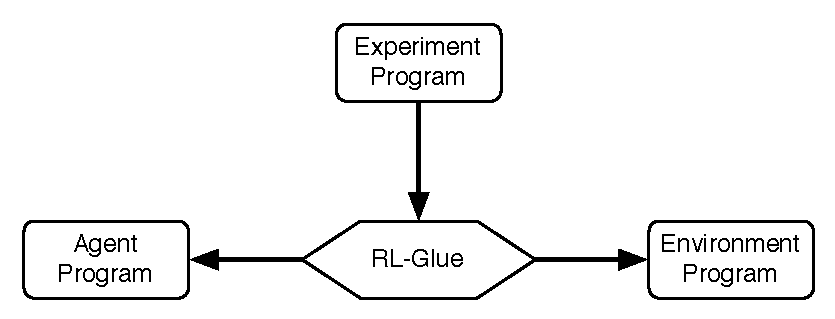
\includegraphics[width=9cm]{glue.pdf}
\vspace{-0.2cm}
\caption{\small The four programs specified by the RL-Glue Protocol.  Arrows indicate the direction of the flow of control.}
\label{fig:RLDIA}
\end{center}
\vspace{-0.4cm}
\end{figure}

 RL-Glue can be used either in  internal or external mode.  In \textit{internal} mode, the agent, environment and experiment are linked into a single program, and their communication is through function calls.  Internal mode is currently an option if the agent, environment, and experiment are written exclusively in Java or C/C++.  In  \textit{external} mode, the agent, environment and experiment are linked into separate programs.  Each program connects to the RL-Glue server program, and all communication is over TCP/IP socket connections. The external mode allows these programs to be written in any programming language that supports socket communication.  External mode is currently supported for C/C++, Java, Python, Lisp, and Matlab.

Each mode has its strengths and weaknesses. Internal mode has less overhead, so it can execute more steps per second. External mode is more flexible and portable.  The performance difference between the two modes vanishes as the agent or environment becomes complex such that computation dominates the socket overhead in terms of time per step.  The agent and environment are indifferent and unaware of their execution mode: the difference in modes lies only in how the agent and environment are linked or loaded.

\section{RL-Glue in Practice}
RL-Glue has provided a common interface for a number of software and hardware projects in the reinforcement-learning community.  For example, there is an annual competition,\footnote{\url{http://www.rl-competition.org/}} where teams from around the world compare their agents on a variety of challenging environments.  The competition software uses an API\footnote{\url{http://code.google.com/p/rl-viz/}} that is layered on top of RL-Glue to dynamically load agent and environment programs, modify parameters at runtime and visualize interaction and performance.  All of the environments and sample agents created by the competition organizers are added to the RL-Library,\footnote{\url{http://library.rl-community.org/}} a public, community-supported repository of RL-Glue compatible code. The RL-Library is also available as a showcase and archive of top competition agents, challenge problems, project code that has been used in academic publications, or any other RL-Glue compatible software that members of our community would like to share.


The socket architecture of RL-Glue allows diverse software and hardware platforms to be connected as RL-Glue environment programs.  There are ongoing projects that connect a mobile robot platform,\footnote{\url{http://www.cs.ualberta.ca/~sokolsky/critterbot/}} a  keepaway soccer server, a real-time strategy game, and an Atari emulator to RL-Glue. Our socket architecture helps lower the barriers for researchers wishing to work on larger scale environments by providing a simple and familiar interface. %These environments will soon be accessible via RL-Library. 

RL-Glue has been used for teaching reinforcement learning in several university courses and to create experiments for scientific articles published in leading conferences. We maintain an updated list\footnote{\url{http://glue.rl-community.org/rl-glue-in-practice}} of all known projects that have benefited from RL-Glue.



\section{Other Reinforcement-Learning Software Projects}
RL-Glue is not the first software project that aims to  standardize empirical reinforcement learning or to make agent and environment programs more accessible within our community.  However, RL-Glue is the only project that offers a standardized language-independent interface, rich actions and observations, and fine-grained control of the experiment.

Other projects, most notably: CLSquare,\footnote{\url{http://www.ni.uos.de/index.php?id=70}}  PIQLE,\footnote{\url{http://piqle.sourceforge.net/}} RL Toolbox,\footnote{\url{http://www.igi.tugraz.at/ril-toolbox/}
} JRLF,\footnote{\url{http://mykel.kochenderfer.com/jrlf/}}  and LibPG,\footnote{\url{http://code.google.com/p/libpgrl/}} offer significant value to the reinforcement-learning community by offering agents and environments, intuitive visualizations, programming tools, etc.  Users should not be forced to choose between RL-Glue and these alternative projects. Our design makes it relatively easy to interface existing frameworks with RL-Glue.  We are currently offering our assistance in bridging other frameworks to RL-Glue, with the hope of improving access to all of these tools for all members of our community.





 
 
 
\section{RL-Glue Open Source Project}
\begin{tabular}{ l l }
  Website &  \url{http://glue.rl-community.org} \\
  License & Apache 2.0  \\
\end{tabular}
\newline
\newline
RL-Glue is more than an interface; it connects a family of community projects, with many levels of possible participation. Members of the community are invited to submit agent, environment and experiment programs to the RL-Library. Developers can also extend the reach of RL-Glue compatibility by writing external or internal -mode interfaces for their favorite programming language.  The RL-Glue Software project also welcomes code submissions and improvements for all parts of the code base.  

% The RL-Glue Software Project has received significant contributions at many of the levels discussed above. The Lisp socket code was contributed by Gabor Balazs. Jose Antonio Martin H. developed a native windows implementation of the RL-Glue Software. The RL-Library has also received several environments submitted from previous competitions participants and paper authors.
%Webpage detailing project contributions?
%Brian: That's a good idea. Very good.

%Brian: Obviously, this is  WAY out of place.



\section{Acknowledgements}
We would like to thank all of the users, testers, and developers for their contributions to RL-Glue 3.0. Special thanks to 
G\'{a}bor Bal\'{a}sz,  %get the accents right
Jos\'{e} Antonio Martin H.,  %get the accents right
Scott Livingston, %Middle Initial?
Marc Bellemare, 
Istv\'{a}n Szita,  %get the accents right
Marc Lanctot, 
Anna Koop, 
Dan Lizotte,
Richard Sutton,
Monica Dinculescu,
Jordan Frank, and
Andrew Butcher.  Of course, we also owe a great debt to all of the talented people responsible for the historic and ongoing development of RL-Glue.\footnote{\url{http://glue.rl-community.org/contributors-history}}

%\addcontentsline{toc}{chapter}{Bibliography}
     %add the above line to get "Bibliography" in the table of contents.
%
%\singlespacing % optional;  Bibliography is better in single spacing
               %            but you may choose different
               %            Don't use \singlespacing if your thesis
               %            is already in single spacing
%
                          % for long bibs.


\bibliographystyle{natbib}
\bibliography{jmlrTake2}



\end{document}  
